\documentclass{scrartcl}

\usepackage{url}
\usepackage{graphicx}
\usepackage{amsmath}
\usepackage{varwidth}
\usepackage[dvipsnames]{xcolor}
\usepackage{algorithm}
\usepackage{algpseudocode}
\usepackage{listings}
\lstset{
	basicstyle=\footnotesize\ttfamily,
	tabsize=4,
	showstringspaces=false,
	breaklines=true,
	prebreak={\space\hbox{\textcolor{Gray}{$\hookleftarrow$}}},
	language=C++
}
\usepackage{enumitem}

\makeatletter
\@addtoreset{section}{part}
\makeatother  

\title{Worksheet 4}
\subtitle{COMP110: Principles of Computing}
\author{Ed Powley}
\date{January 2016}

\renewcommand\thepart{\Alph{part}}

\begin{document}

\maketitle

\section*{Introduction}

In this assignment, you will create three small C++ programs:
\begin{enumerate}[label=\Alph*.]
	\item A console application implementing the word guessing game Hangman;
	\item A console application implementing the 2-player strategy game Connect~4;
	\item A graphical application which generates and displays the Mandelbrot fractal.
\end{enumerate}

This worksheet tests your ability to translate various program notations (pseudocode, flowcharts,
mathematics, narrative descriptions) into C++ code.

\section*{Submission instructions}

The GitHub repository at the following URL contains skeleton projects for the three parts of this worksheet.
\begin{center}
\url{https://github.com/Falmouth-Games-Academy/comp110-worksheet-4}
\end{center}
Fork this repository into your own GitHub account. To submit, create a GitHub pull request.

For the most part, this worksheet requires you to edit C++ code in the skeleton projects provided.
\textbf{Please do not rename or delete the projects or files provided, and please do not create new projects.}
For those questions which require you to produce artefacts other than C++ code, e.g.\ pseudocode or flowcharts,
this material should be formatted in Markdown (possibly with embedded images) and added to your GitHub repository.

Information on using GitHub is available on LearningSpace, and elsewhere online.

\section*{Marking}

\subsection*{Timely submission: $40\%$}

To obtain the marks for timely submission, you must submit Part~A by \textbf{6pm, Monday 18th January},
\textbf{and} Parts~B and~C by \textbf{6pm, Monday 8th February}.
As with other worksheets, you may resubmit after these deadlines in order to address any correctness issues
or satisfy further quality criteria. This $40\%$ is awarded as long as you submit \emph{something} by the deadline.

\subsection*{Correctness: $30\%$}

To obtain the marks for correctness, you must submit working solutions for the following:
\begin{itemize}
\item Part~A, Sections~\ref{core-a-first}--\ref{core-a-last};
\item Part~B, Sections~\ref{core-b-first}--\ref{core-b-last};
\item Part~C, Sections~\ref{core-c-first}--\ref{core-c-last}.
\end{itemize}
Note that this is a threshold: the full $30\%$ is awarded for work which is \emph{complete}
and contains \emph{no clear errors}. In particular you will not be penalised for trivial errors which do not
affect the overall functioning of your programs, nor will you receive extra credit for highly polished solutions.

\subsection*{Quality: $30\%$}

The extra quality criteria for this worksheet are as follows:
\begin{enumerate}
\item\textbf{Part A stretch goal.} You have submitted a working solution for Part~A, Section~\ref{stretch-a}.
\item\textbf{Part B stretch goal.} You have submitted a working solution for Part~B, Section~\ref{stretch-b}.
\item\textbf{Part C stretch goal.} You have submitted a working solution for Part~C, Section~\ref{stretch-c}.
\item\textbf{Presentation.} Your solutions are appropriately presented in GitHub, with descriptive commit messages
	and appropriate documentation in \texttt{readme.md} files.
	You have edited the provided skeleton projects, and refrained from renaming the provided files or creating new projects.
\item\textbf{Sophistication.} Your solution for \textbf{any one} of the stretch goals is particularly sophisticated,
	demonstrating mastery of C++ programming concepts appropriate to the task at hand.
\end{enumerate}

\clearpage
\part{Hangman}

In this part, you will implement a basic Hangman\footnote{\url{https://en.wikipedia.org/wiki/Hangman_(game)}} game.
The provided skeleton project contains code for reading a list of words from a text file, and choosing one at random.
You will implement the rest of the game.

\section{} \label{core-a-first}

\textbf{Implement} a function \lstinline{char getLetter()} which does the following:
\begin{enumerate}
\item \label{hangman:step1} Prompt the user to enter a letter.
\item Get a line of input from the console, and take the first character.
\item If the character is a letter, convert it to upper case and return it.
\item Otherwise, display an error and go to step~\ref{hangman:step1}.
\end{enumerate}

You may find the following functions useful: \lstinline{isalpha}, \lstinline{toupper}, and \lstinline{std::getline}.
Look online for details of how to use them.

\section{}

\textbf{Implement} the following algorithm as a C++ function.
The algorithm takes the current partially revealed word, the secret word, and a guessed letter.
It returns a new partially revealed word, in which the guessed letter has been filled in where it appears in the string.

\begin{algorithm}
\begin{algorithmic}
	\Procedure{FillInLetter}{partialWord, secretWord, letter}
		\State $\text{result} \gets \text{empty string}$
		\For{$i = 0, 1, \dots, \text{secretWord.length} - 1$}
			\If{$\text{secretWord}[i] = \text{letter}$}
				\State append letter to result
			\Else
				\State append $\text{partialWord}[i]$ to result
			\EndIf
		\EndFor
		\State \textbf{return} result
	\EndProcedure
\end{algorithmic}
\end{algorithm}

The following table gives some examples of possible input and output:

\begin{center}
\begin{tabular}{|ccc|c|}
\hline
partialWord & secretWord & letter & result \\ \hline
\lstinline{"B-----"} & \lstinline{"BANANA"} & \lstinline{'A'} & \lstinline{"BA-A-A"} \\ \hline
\lstinline{"B-----"} & \lstinline{"BANANA"} & \lstinline{'E'} & \lstinline{"B-----"} \\ \hline
\lstinline{"-----"} & \lstinline{"APPLE"} & \lstinline{'L'} & \lstinline{"---L-"} \\ \hline
\lstinline{"-----"} & \lstinline{"APPLE"} & \lstinline{'B'} & \lstinline{"-----"} \\ \hline
\end{tabular}
\end{center}

\section{} \label{core-a-last}

\textbf{Implement} a playable Hangman game, using the functions implemented above and structured
according to the following flowchart:

\begin{center}
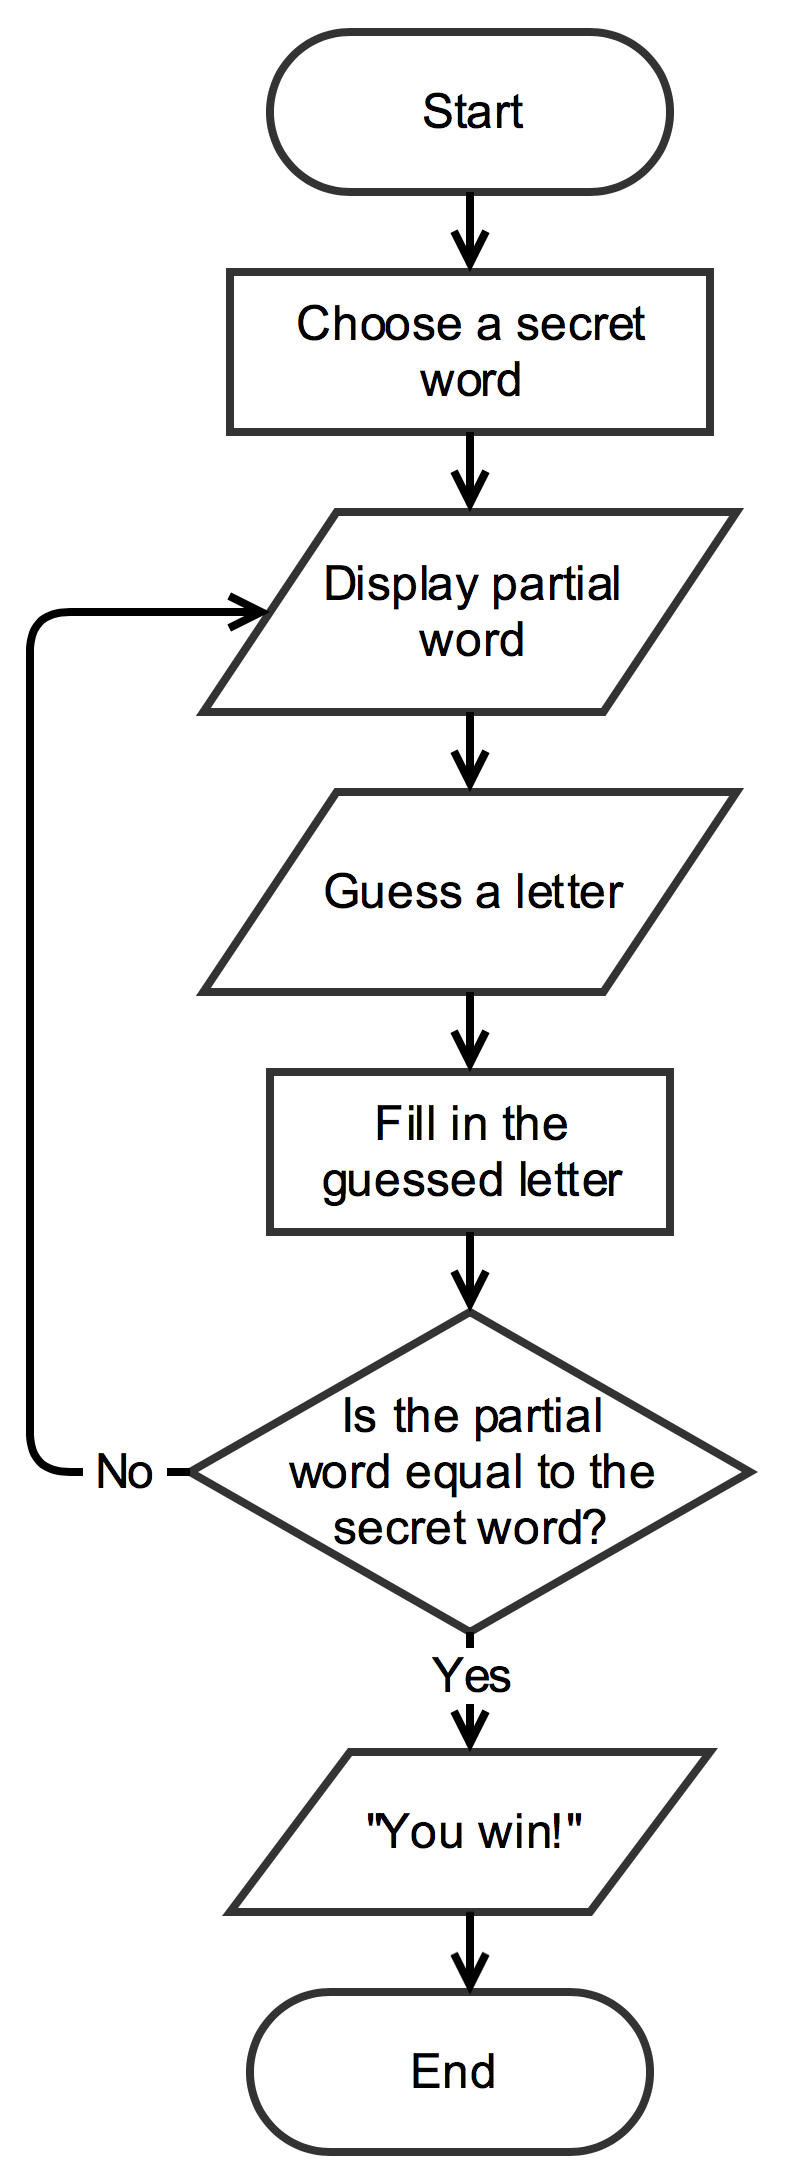
\includegraphics[height=0.5\textheight]{hangman_flowchart.png}
\end{center}

\section{Stretch goal} \label{stretch-a}

The game would be more interesting if the player had a limited number of lives in which to guess the word,
and lost a life for guessing a letter which was not present in the word.

\textbf{Modify} the flowchart above to make this change. \textbf{Modify} your C++ program to reflect your revised flowchart.

\clearpage
\part{Connect 4}

\section{}
Do a thing

\section{}
Do another thing

\clearpage
\part{Mandelbrot}

\section{}

\textbf{Implement} the following algorithm in C++. Use a \lstinline{switch} statement,
taking advantage of the fact that casting a \lstinline{double} to an \lstinline{int} causes it to be rounded down.
The \lstinline{abs} and \lstinline{fmod} functions are defined in \lstinline{<math.h>}.

\begin{algorithm}
\begin{algorithmic}
	\Procedure{HSVtoRGB}{$h, s, v$}
		\State $c \gets s \times v$
		\State $h' = 6 \times h$
		\State $x \gets c \times \left(1 - \operatorname{abs} \left( \operatorname{fmod} \left( h', 2 \right) - 1 \right) \right)$
		\If{$0 \leq h' < 1$}     \State $r = c$; $g = x$; $b = 0$
		\ElsIf{$1 \leq h' < 2$}  \State $r = x$; $g = c$; $b = 0$
		\ElsIf{$2 \leq h' < 3$}  \State $r = 0$; $g = c$; $b = x$
		\ElsIf{$3 \leq h' < 4$}  \State $r = 0$; $g = x$; $b = c$
		\ElsIf{$4 \leq h' < 5$}  \State $r = x$; $g = 0$; $b = c$
		\ElsIf{$5 \leq h' < 6$}  \State $r = c$; $g = 0$; $b = x$
		\Else                    \State $r = 0$; $g = 0$; $b = 0$
		\EndIf
		\State \textbf{return} $(r+v-c,\ g+v-c,\ b+v-c)$
	\EndProcedure
\end{algorithmic}
\end{algorithm}

This algorithm converts a colour in HSV space to the equivalent colour in RGB space;
all of $r,g,b,h,s,v$ are assumed to be between $0$ and $1$.

\end{document}
